\documentclass[letter]{article}
\usepackage{amsmath}
\usepackage{amsfonts}
\usepackage{amssymb}
\usepackage{ifthen}
\usepackage{enumitem}
\usepackage{fancyhdr}
\usepackage[hidelinks]{hyperref}
\usepackage{xcolor}
\usepackage{tikz}
\hypersetup{
    colorlinks,
    linkcolor={red!50!black},
    citecolor={blue!50!black},
    urlcolor={blue!80!black}
}

\definecolor{deepblue}{rgb}{0,0,0.5}
\definecolor{deepred}{rgb}{0.6,0,0}
\definecolor{deepgreen}{rgb}{0,0.5,0}

\usepackage{listings}

% Default fixed font does not support bold face
\DeclareFixedFont{\ttb}{T1}{txtt}{bx}{n}{12} % for bold
\DeclareFixedFont{\ttm}{T1}{txtt}{m}{n}{12}  % for normal

% Python style for highlighting
\newcommand\pythonstyle{\lstset{
language=Python,
basicstyle=\ttm,
otherkeywords={self},             % Add keywords here
keywordstyle=\ttb\color{deepblue},
emph={MyClass,__init__},          % Custom highlighting
emphstyle=\ttb\color{deepred},    % Custom highlighting style
stringstyle=\color{deepgreen},
frame=tb,                         % Any extra options here
showstringspaces=false            % 
}}


% Python environment
\lstnewenvironment{python}[1][]
{
\pythonstyle
\lstset{#1}
}
{}

% Python for external files
\newcommand\pythonexternal[2][]{{
\pythonstyle
\lstinputlisting[#1]{#2}}}

% Python for inline
\newcommand\pythoninline[1]{{\pythonstyle\lstinline!#1!}}


%%%
% Set up the margins to use a fairly large area of the page
%%%
\oddsidemargin=.0in
%\evensidemargin=.2in
\textwidth=6.5in
\topmargin=0in
\textheight=8.75in
\parskip=.07in
\parindent=0in
\pagestyle{fancy}

%%%
% Set up the header
%%%
\newcommand{\setheader}[6]{
	\lhead{{\sc #1}\\{\sc #2}}% ({\small \it \today})}
	\rhead{
		{\bf #3} 
		\ifthenelse{\equal{#4}{}}{}{(#4)}\\
		{\bf #5} 
		\ifthenelse{\equal{#6}{}}{}{(#6)}%
	}
}

\makeatletter
\newcommand{\escapeus}{\begingroup\@makeother\_\@escapeus}
\newcommand*{\@escapeus}[1]{#1\endgroup}
\makeatother

%%%
% Set up some shortcut commands
%%%
\newcommand{\R}{\mathbb{R}}
\newcommand{\N}{\mathbb{N}}
\newcommand{\Z}{\mathbb{Z}}
\newcommand{\Proj}{\mathrm{proj}}
\newcommand{\Perp}{\mathrm{perp}}
\newcommand{\proj}{\mathrm{proj}}
\newcommand{\Span}{\mathrm{span}}
\newcommand{\Null}{\mathrm{null}}
\newcommand{\Rank}{\mathrm{rank}}
\newcommand{\mat}[1]{\begin{bmatrix}#1\end{bmatrix}}
\newcommand{\var}[1]{{$\langle$\it #1$\rangle$}}
\newcommand{\Code}[1]{\texttt{\escapeus #1}}

%%%
% This is where the body of the document goes
%%%
\begin{document}
	\setheader{APM348}{Homework 3}{Due: 5:59pm March 9}{}{}{}


In this homework assignment you will use \verb|python| to solve the ordinary differential equation associated with the SIR compartment model for the spread of a disease. You will study how the disease spreads across a network of populations

Clone the file \href{https://utoronto.syzygy.ca/jupyter/user-redirect/git-pull?repo=https://github.com/bigfatbernie/IBLMathModeling&subPath=homeworks/homework3/homework3-exercises.ipynb}{\tt homework3-exercises.ipynb} into your Jupyter Notebook and solve the exercises directly there. \\

You must submit two PDF files to gradescope:
\begin{itemize}
	\item A \LaTeX'ed document in PDF format with your answers and conclusions to the problem, referencing the python code and citing all sources used.
	\item A PDF document from exporting your Jupyter Notebook
\end{itemize}



\section{A Network SIR Model}


When modelling the global spread of disease, the assumption of a well-mixed population is often called into question. People are not totally free to mix between countries. We will address this concern by simulating a network of populations. You should view each population as a well-mixed country and the network connections represent the travel permitted between countries.


In the network of populations, each population has its own $S$, $I$, and $R$. We will index them with $i$. For generality, we will allow the parameters $\beta$ and $\gamma$ to vary from population to population. The dynamics are

\begin{align}
	\frac{dS_i}{dt} & = -\beta_i S_i I_i + \sum_{j} T^S_{i,j} S_j - \sum_j T^S_{j,i} S_i, \label{SIR:S}\\
	\frac{dI_i}{dt} & = 	\beta_i S_i I_i - \gamma_i I_i + \sum_{j} T^I_{i,j} I_j - \sum_j T^I_{j,i} I_i, \label{SIR:I} \\
	\frac{dR_i}{dt} & = \gamma_i I_i + \sum_{j} T^R_{i,j} R_j - \sum_j T^R_{j,i} R_i \label{SIR:R}
\end{align}

The coefficients $T^S_{i,j}$, $T^I_{i,j}$, and $T^R_{i,j}$ are the travel rates from population $j$ and to population $i$ for the susceptibles, infectives, and recovereds respectively. Note that the susceptibles from one population become the susceptibles in another and likewise for infectives and recovereds. The travel rates of the susceptibles, infectives, and recovereds can be different. The positive travel terms correspond to people entering population $i$ from each other population (sum over $j$). The negative travel terms correspond to people leaving population $i$ to each other population (sum over $j$). Note that the subscripts $i$ and $j$ have changed positions. These travel rates determine if travel is possible (a non-zero value) and how frequently travel occurs. Note that the total global population $\displaystyle N = \sum_i (S_i + I_i + R_i)$ is conserved.



\section{Assignment}

\begin{enumerate}[label=\textbf{\arabic*.}]
	\item \label{onepop}On the notebook \href{https://utoronto.syzygy.ca/jupyter/user-redirect/git-pull?repo=https://github.com/bigfatbernie/IBLMathModeling&subPath=homeworks/homework3/homework3-exercises.ipynb}{\tt homework3-exercises.ipynb}, 
	%	Download the Matlab program one population.m. 
	read the code and comments of the first part to determine how it works. The core of the program is the call to \verb|ode45| to solve the ordinary differential equation. Note that I have been vague about the units. By setting $\gamma = 1$, I am essentially saying that my unit of time is $1/\gamma$, the typical time for an infected individual to recover. The population sizes should be compared against the total population of $N$ and interpreted as fractions of the population.
	
	\item Run the program that simulates one population. Reduce the value of $\beta$ and note the reduction in the size of the outbreak in both the maximum number of infected and the terminal number of recovereds. Modify the initial condition so that there are initially more infective individuals (reduce the size of the initial susceptibles so that the total population size is the same). How does this affect the size of the outbreak?

	\item Observe the second part of the notebook and how the 
	% Download the Matlab program SIRpopulations.m. Observe how the 
	differential equations are entered in the right-hand side function in \verb|multipopulation_sir_rhs|. 
	Run the program and make sure you understand the output plots. The top panel shows the distribution of the populations over time. The first population is on the bottom of the stacked area curves. The pie chart shows the sizes of the compartments. Moving counter- clockwise, the $S$, $I$, and $R$ values for each population (if they are large enough) are shown as fractions of the global population at a sequence of times. After the animation finishes, a table of the final global distribution is shown.
	
	\item Set all of the travel rates to zero ($T_{\rm none}$) and observe that the populations behave independently and compare it to the result of Exercise \ref{onepop} 
	Set the travel rates using one of the provided structures (circle, a chain, all-to-all, etc) and validate that the output makes sense.

	\item Describe two different assumptions in the model of travel implicit in Eqs. \eqref{SIR:S}--\eqref{SIR:R}.

	\item When only susceptibles can travel, how are the long-run numbers of recovereds in the network of populations different than that for one population? Set all of the $\gamma$ equal to $1$ and the $\beta$ equal to $2.0/6000$. For each provided network structure for the susceptibles travel rates (set the others to none) and each of the numbers of populations from 1 to 6, report using a table the percentage of recovereds in steady-state. Keep the total global population at 6000 and use equal initial population sizes. Explain anything that you find interesting. Refer to $R_0$ in your explanation.
		
	\item How does travel of infectives spread the disease? Consider four populations with the original $\gamma$ and $\beta$ and no travel for susceptibles or recovereds. Reduce the base travel rate to $\nu = 0.01$. You may need to increase the final time of the simulation to find the steady state. For each provided network structure, report the final distribution of recovereds and discuss the time courses of the disease spread. Can population 3, with its lower $R_0$, prevent the spread of the disease in the one direction circular network? How does the time delay between outbreaks reveal the travel network structure?
	


	
	
\end{enumerate}

\newpage

\section{Numerical Approximation of the Heat Equation}

In this part of the homework assignment, you will approximate the steady-state temperature of a 2-dimensional object.

For that, first consider the steady-state heat equation:
\begin{equation}\tag{H}\label{HeatEq}
	\Delta u = u_{xx} + u_{yy} = \frac{\partial^2 u}{\partial x^2} + \frac{\partial^2 u}{\partial y^2} = 0,
\end{equation}
where $\Delta u$ is called the Laplacian of $u$ and $u(x,y)$ is the temperature of the 2-dimensional slab at the position $(x,y)$ in Celsius.

We also assume that we know the temperature of the 2-dimensional object on the edges.

We will use the main idea of Euler's method to approximate the solution to this problem.


\begin{enumerate}[resume, label=\textbf{\arabic*.}]
	\item The main idea of Euler's method is to discretize the derivative of a function:
	\[ y'(t_n) \approx \frac{y(t_{n+1}) - y(t_n)}{\delta t} \]
	
	Use this idea to obtain a discretized version of $y''(t_n)$.
	
	
	\item Now consider the domain $0 \leq x \leq L$ and $0 \leq y \leq H$.
	\begin{center}
	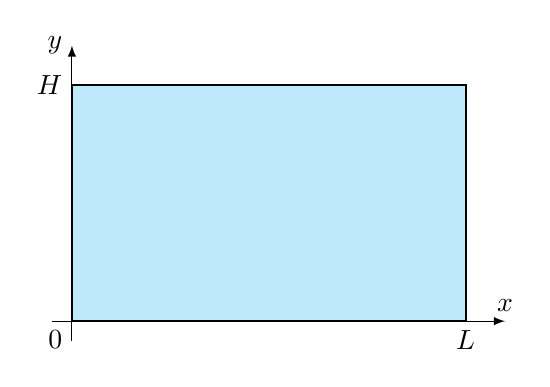
\begin{tikzpicture}
		\draw[-latex] (-0.25,0) -- (5.5,0) node[above] {$x$};
		\draw[-latex] (0,-0.25) -- (0,3.5) node[left] {$y$};
		\draw (0,0) node[below left] {$0$};
		\draw (5,0) node[below] {$L$};
		\draw (0,3) node[left] {$H$};
		\draw[thick, fill=cyan!25!white] (0,0) -- (5,0) -- (5,3) -- (0,3) -- cycle;
	\end{tikzpicture}	
	\end{center}

	Consider the points $x_i = i \Delta x$ and $y_j = j \Delta y$ and the approximation $u_{ij} \approx u(x_i ,y_j)$.
	
	Write a discretized formula for $u_{xx}(x_i,y_j)$ in terms of $u_{ij}$. Do the same for $u_{yy}(x_i,y_j)$.
	
	\item Using these, obtain a numerical scheme for \eqref{HeatEq}.

	\item This scheme is \textit{implicit}, so we need to find a way to solve it.
	
	For that, consider $L=4, H=4$ and the following boundary conditions:
	\begin{itemize}
		\item $u(x,0) = u(0,y) = 0$
		\item $u(4,y) = 50$
		\item $u(x,3) = 100$
	\end{itemize}
	
	What do they mean in practice?
	
	\item Consider $\Delta x = \Delta y = 1$ and the following definition of points:
		\begin{center}
	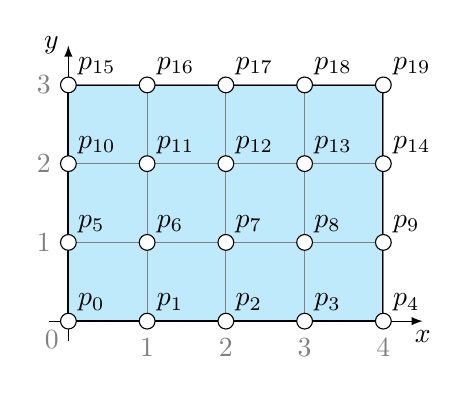
\begin{tikzpicture}
		\draw[-latex] (-0.25,0) -- (4.5,0) node[below] {$x$};
		\draw[-latex] (0,-0.25) -- (0,3.5) node[left] {$y$};
		\draw[thick, fill=cyan!25!white] (0,0) -- (4,0) -- (4,3) -- (0,3) -- cycle;
		\draw[gray] (0,0) node[below left] {$0$};
		\foreach \i in {1, 2, 3, 4} {
		  \draw[gray] ({\i}, 3) -- ({\i},-0.1) node[below] {${\i}$};
		}
		\foreach \j in {1, 2, 3} {
		  \draw[gray] (4, {\j}) -- (-0.1,{\j}) node[left] {${\j}$};
		}
		\foreach \i in {0, ..., 19} {
		  \draw[fill=white] ({int(mod(\i,5))},{int(\i/5)}) circle (0.1) node[above right] {$p_{\i}$};
		}
		
	\end{tikzpicture}	
	\end{center}

	Consider the approximate solution vector:
	\[ \vec{u} = 
		\mat{u(p_0) \\ u(p_1) \\ \vdots \\ u(p_{19}) }
	\]

	Write the numerical scheme found above as a system for $\vec{u}$
	\[
	A \vec{u} = \vec{b}.
	\]
	
	Explain how you can reduce it to a $6 \times 6$ system.
	
	Use \verb|python| to solve the $6\times 6$ system and sketch the solution.
	
	\item Consider the same problem with $N_x$ and $N_y$ points on the horizontal and vertical directions, and consider $\Delta x = \frac{4}{N_x}$ and $\Delta y = \frac{3}{N_y}$.
	
		Solve the system and sketch its solution for $\Delta x = \Delta y = 0.1$.
		
	\item \textbf{(Bonus)} Solve the system and sketch a solution for the same problem with the domain
		\begin{center}
		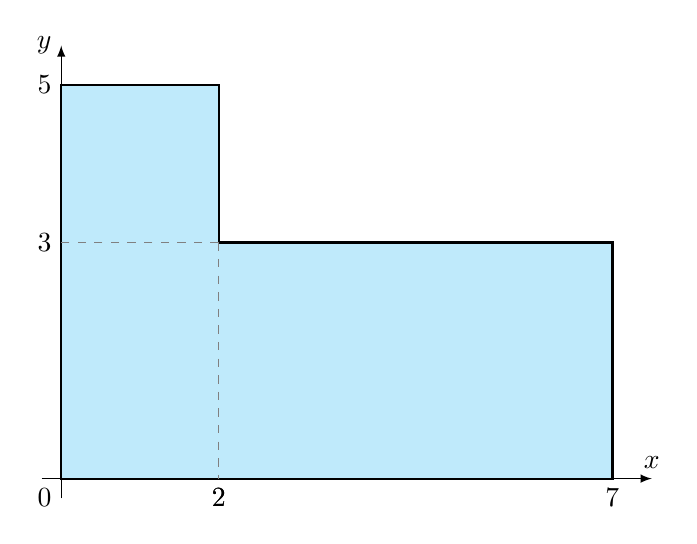
\begin{tikzpicture}
			\draw[-latex] (-0.25,0) -- (7.5,0) node[above] {$x$};
			\draw[-latex] (0,-0.25) -- (0,5.5) node[left] {$y$};
			\draw[thick, fill=cyan!25!white] (0,5) -- (0,0) -- (7,0) -- (7,3) -- (2,3) -- (2,5) -- cycle;
			\draw (0,0) node[below left] {$0$};
			\draw (7,0) node[below] {$7$};
			\draw (2,0) node[below] {$2$};
			\draw (0,5) node[left] {$5$};
			\draw[gray, dashed] (2,3) -- (2,0) node[below, black] {$2$};
			\draw[gray, dashed] (2,3) -- (0,3) node[left, black] {$3$};
		\end{tikzpicture}	
		\end{center}
		and boundary conditions:
		\begin{itemize}
			\item $u(0,y) = u(x,0) = 0$
			\item $u(x,5) = 10x$
			\item $u(2,y) = 70-10y$ for $3 \leq y \leq 5$
			\item $u(x,3) = 20+10x$ for $2 \leq x \leq 6$
			\item $u(5,y) = 30x$
		\end{itemize}
	
		Use small values of $\Delta x$ and $\Delta y$ so the graph looks good.
	
\end{enumerate}




	
\end{document}  
